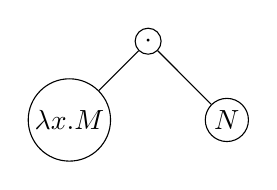
\begin{tikzpicture}[
  level distance=10mm,
  sibling distance=20mm,
  every node/.style={circle,draw,inner sep=1.5pt}
  ]
  \node {$\cdot$}
    child { node {$\lambda x.M$} }
    child { node {$N$} };
\end{tikzpicture}
\qquad$\Longrightarrow$\qquad
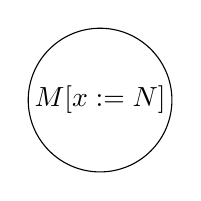
\begin{tikzpicture}[
  level distance=10mm,
  sibling distance=20mm,
  every node/.style={circle,draw,inner sep=1.5pt}
  ]
  \node {$M[x:=N]$};
\end{tikzpicture}
